%! TEX root = ../main.tex
\documentclass[main]{subfiles}

\begin{document}
\section{Introduction}

An elliptic curve defined over a field $K$ of characteristic $\neq 2$ is a curve defined by a Weierstrass equation
\begin{equation*}
    E: y^{2} = x^{3} + Ax^2 + Bx + C
\end{equation*}
where $A,B,C \in K$ and the discriminant $\Delta = -4A^3C + A^2B^2 + 18ABC - 4B^3 - 27C^2$ is nonzero.
On points on an elliptic curve defined over $\mathbb{Q}$, we can define an addition law geometrically.
For two points $P,Q$ on $E$, the point $-(P+Q)$ is defined as the third point of intersection of the line passing through $P$ and $Q$ with the curve.
The sum $P+Q$ is the point symmetric to $-(P+Q)$ with respect to the $x$-axis.
The definition can be extended to any field $K$ of characteristic $\neq 2$.
The set of points on an elliptic curve forms an abelian group with the identity element being the point at infinity.
The Mordell-Weil group $E(K)$ is a group consisting of all $K$-rational points on $E$.
\begin{figure}[H]
    \centering
    \caption{$E: y^2 = x(x-3^2)(x+4^2)$}
    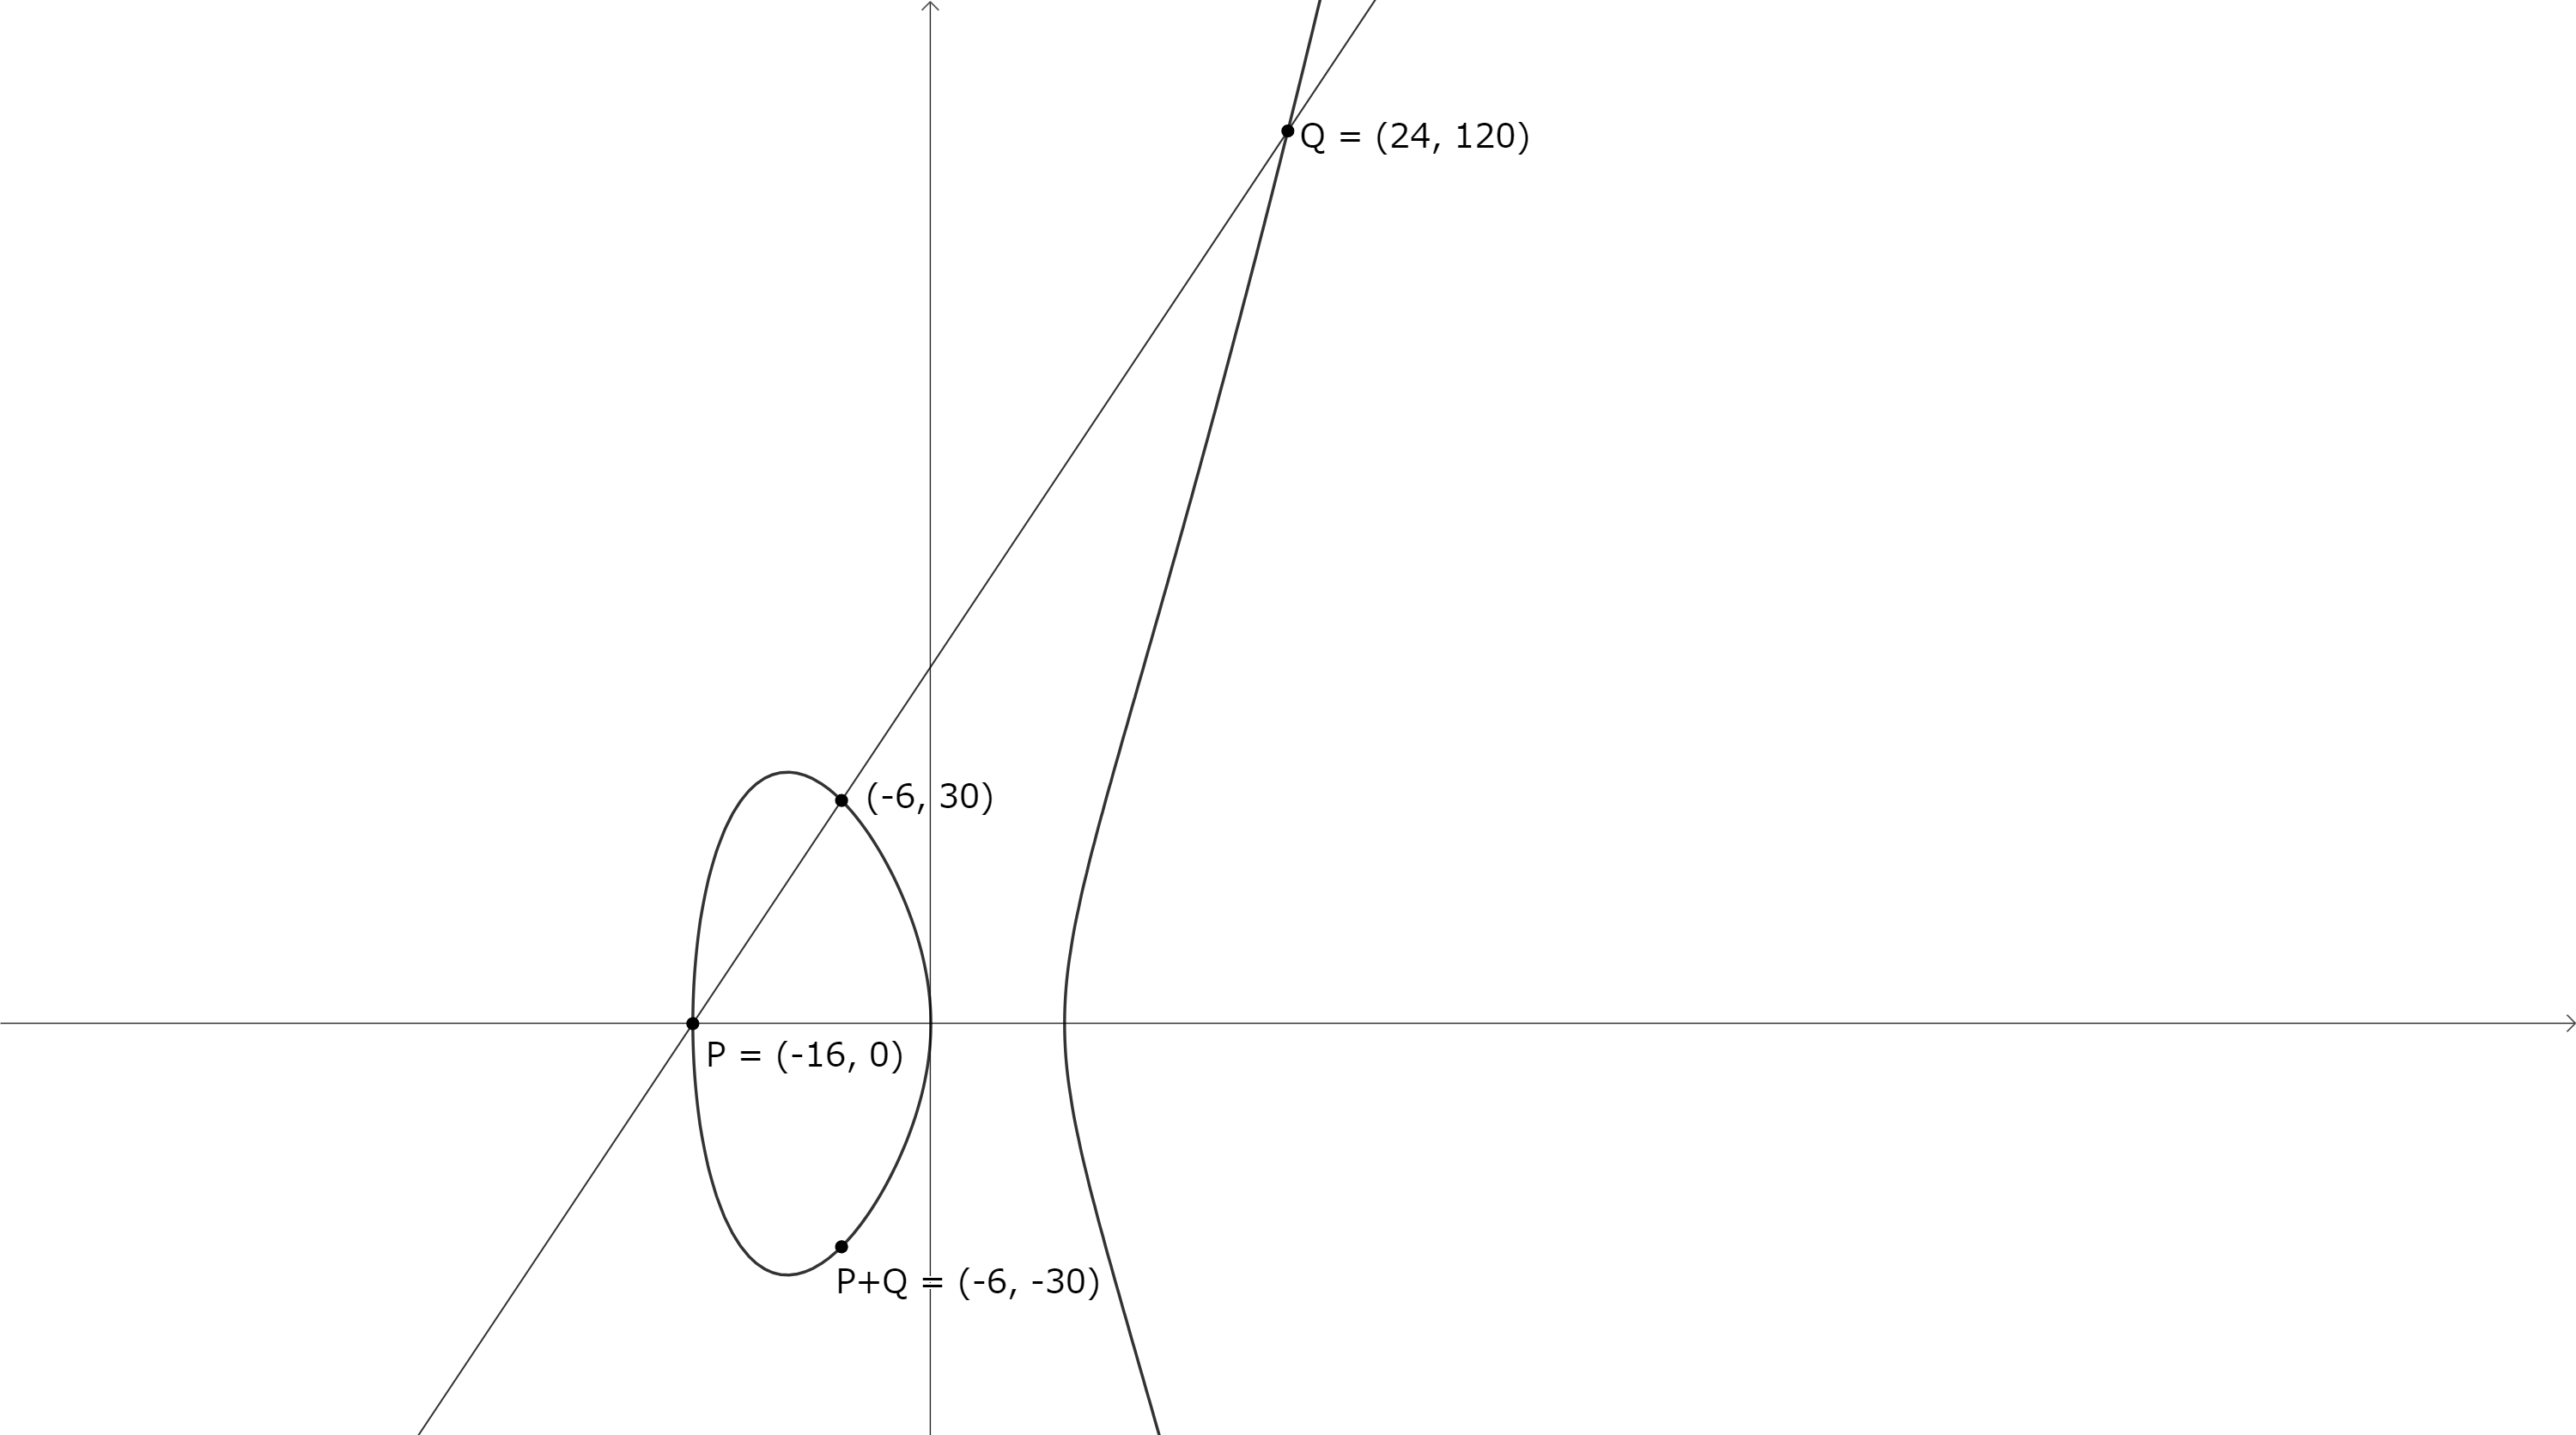
\includegraphics[keepaspectratio, width=0.7\linewidth]{figures/3-4-5.png}
    \label{fig:elliptic_curve}
\end{figure}

\begin{thm}
    The kernel of multiplication by $2$ map $[2]: E(K) \to E(K)$ is
    \begin{equation*}
        E(K)[2] = \{ \mathcal{O} \} \cup \{ (x,y) \in E(K) \mid y = 0 \}.
    \end{equation*}
\end{thm}

\begin{thm}{(Mordell-Weil's Theorem)}
    \label{thm:mordell}
    Let $E$ be an elliptic curve defined over a number field $K$.
    Then the Mordell-Weil group $E(K)$ is a finitely generated abelian group.
\end{thm}
By the structure theorem of finite abelian groups, the Mordell-Weil group can be decomposed into a free part and a torsion part:
\begin{equation*}
    E(K) \cong \mathbb{Z}^{\oplus r} \oplus E(K)_{\text{tors}}
\end{equation*}
where $r$ is the rank of the Mordell-Weil group and $E(K)_{\text{tors}}$ is the torsion subgroup of $E(K)$.
The Mordell-Weil group is an important object in the arithmetic of elliptic curves.
Especially, the rank of the Mordell-Weil group is important and difficult to determine, in general.

Let $a,b,c$ be positive integers which satisfy the Fermat's equation
\begin{equation*}
    a^{n} + b^{n} = c^{n}.
\end{equation*}
for any integer $n \geq 3$ and consider the elliptic curve defined by the Weierstrass equation
\begin{equation*}
    y^{2} = x(x - a^{n})(x + b^{n}),
\end{equation*}
which is called the Frey curve.
The Frey curve played an important role in the proof of Fermat's Last Theorem by Wiles.
Wiles proved that the Frey curves do not exist, which implies that the Fermat's equation has no nontrivial solution.

In this paper, we consider the case $n=2$ of the Frey curves.
In other words, let $(a,b,c) \in \mathbb{Z}^3$ be a Pythagorean triple and consider the elliptic curve defined by the Weierstrass equation
\begin{equation}
    \label{eq:2frey}
    y^{2} = x(x - a^{2})(x + b^{2}),
\end{equation}
which we call the Frey curve of degree $2$.
The Frey curves of degree $2$ do exist infinitely unlike for $n \geq 3$.

We can parameterize Pythagorean triples $(a,b,c)$ by $m,n \in \mathbb{Z}$ with $(m,n)=1$ as $(a,b,c) = (2mn, m^{2} - n^{2}, m^{2} + n^{2})$.
Then the equation \eqref{eq:2frey} can be written as $y^{2} = x(x - 4m^2n^2)(x + (m^{2} - n^2)^{2})$.
We replace $x,y$ by $n^2x, n^3y$ and put $s = m/n$.
Then we get an elliptic curve
\begin{equation}
    \label{eq:E_{1,s}}
    E_{1,s}: y^{2} = x(x - 4s^{2})(x + (s^{2} - 1)^{2}).
\end{equation}
We consider $E_{1,s}$ as an elliptic curve over a function field $\overline{\mathbb{Q}}(s)$.

For any elliptic curves $E$ over a function field $k(C)$ of a smooth irreducible projective curve $C$ over an algebraically closed field $k$, there is an elliptic surface $\pi: \mathcal{E} \to C$ with the generic fiber $E$ called the \Neron{} model.
We can use tools in the theory of surfaces by associating an elliptic surface $\mathcal{E}_{1,s} \to \mathbb{P}^1$ to $E_{1,s}$.

For $s \in \overline{\mathbb{Q}}$, $\mathcal{E}_s:=\pi^{-1}(s)$ is called the special fiber at $s$.
For all but finitely many $s \in \overline{\mathbb{Q}}$, the special fiber $\mathcal{E}_s$ at $s$ is non-singular, which means that $\mathcal{E}_s$ is an elliptic curve.

The Mordell's Theorem also holds for elliptic curves over a function field.
\begin{thm}{(\cite[Theorem 6.1.]{ref:advancedaec})}
    \label{thm:mordell_function_field}
    Let $\mathcal{E} \to C$ be an elliptic surface defined over a field $k$ and $E$ be the corresponding elliptic curve over the function field $k(C)$.
    If $\mathcal{E} \to C$ does not split, then the Mordell-Weil group $E(k(C))$ is a finitely generated abelian group.
\end{thm}

On the relation between the Mordell-Weil group of an elliptic curve over a function field and its special fibers, the following theorem is known.
We can reduce results obtained by treating a family of elliptic curves uniformly as an elliptic surface to results for each elliptic curve.
\begin{thm}{(Specialization Theorem, \cite[Theorem 11.4.]{ref:advancedaec})}
    \label{thm:specialization}
    Let $\mathcal{E} \to C$ be a non-split elliptic surface defined over a number field $k$ and $E$ be the corresponding elliptic curve over the function field $k(C)$.
    Let $k'=k$ or $\overline{k}$ where $\overline{k}$ is the algebraic closure of $k$.
    Then for all but finitely many $s \in C(k')$, a homomorphism
    \begin{equation*}
        E(k(C)) \hookrightarrow \mathcal{E}_{s}(k'),
    \end{equation*}
    called the specialization homomorphism at $s$, is injective.
\end{thm}

\begin{lem}{(\cite[Exercise 3.9.(a)]{ref:advancedaec})}
    Let $\mathcal{E}$ be an elliptic surface over $k$, and let $j_{\mathcal{E}}: C \to \mathbb{P}^1$ be a morphism such that $j_{\mathcal{E}}(v)$ gives the $j$-invariant for any non-singular fibers $\mathcal{E}_v$.
    If $\mathcal{E}$ splits over $k$, then $j_{\mathcal{E}}$ is a constant map.
\end{lem}

\begin{rem}
    All elliptic surfaces appearing in this paper have non-constant $j$-invariants, therefore, they do not split.
    Thus we can apply the Specialization Theorem (Theorem~\ref{thm:specialization}).
\end{rem}

\end{document}